\chapter{Background}

\section{Sicurezza Industriale e DPI}

La sicurezza sul lavoro nell'industria manifatturiera è di primaria importanza per garantire non solo la salute e il benessere dei lavoratori, ma anche l'efficienza operativa e la sostenibilità economica delle aziende. Secondo i dati forniti dall'Istituto Nazionale per l'Assicurazione contro gli Infortuni sul Lavoro (INAIL), nel 2022 il settore manifatturiero ha registrato un tasso di infortuni del 13,9\% sul totale \cite{inail2023}.

\begin{figure}[htbp]
    \centering
    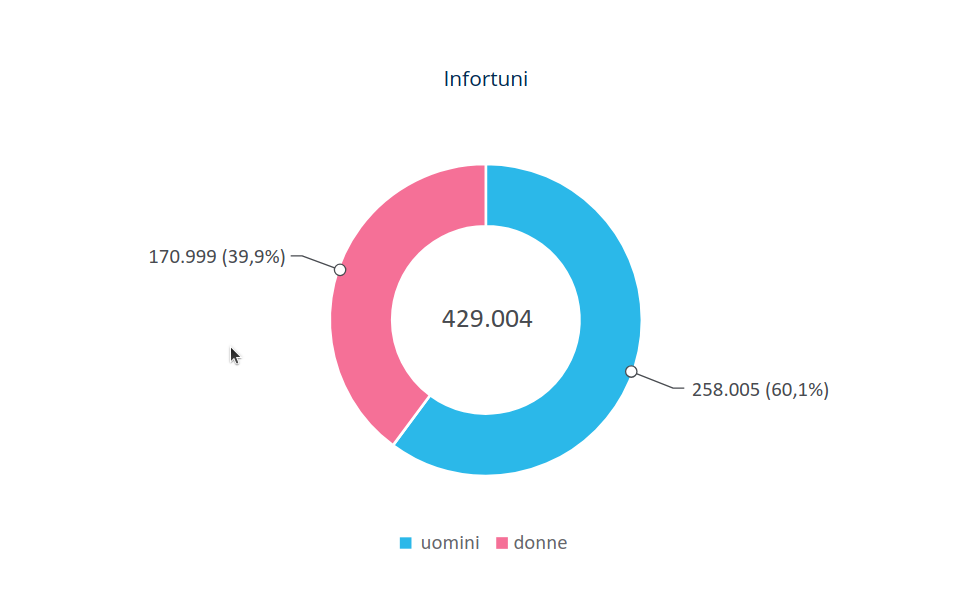
\includegraphics[width=0.8\textwidth]{figures/totaleinfortuni.png}
    \caption{Infortuni sul lavoro accertati positivi per genere
e modalità di accadimento nell'anno 2022.}
    \label{fig:infortot}
\end{figure}

\begin{figure}[htbp]
    \centering
    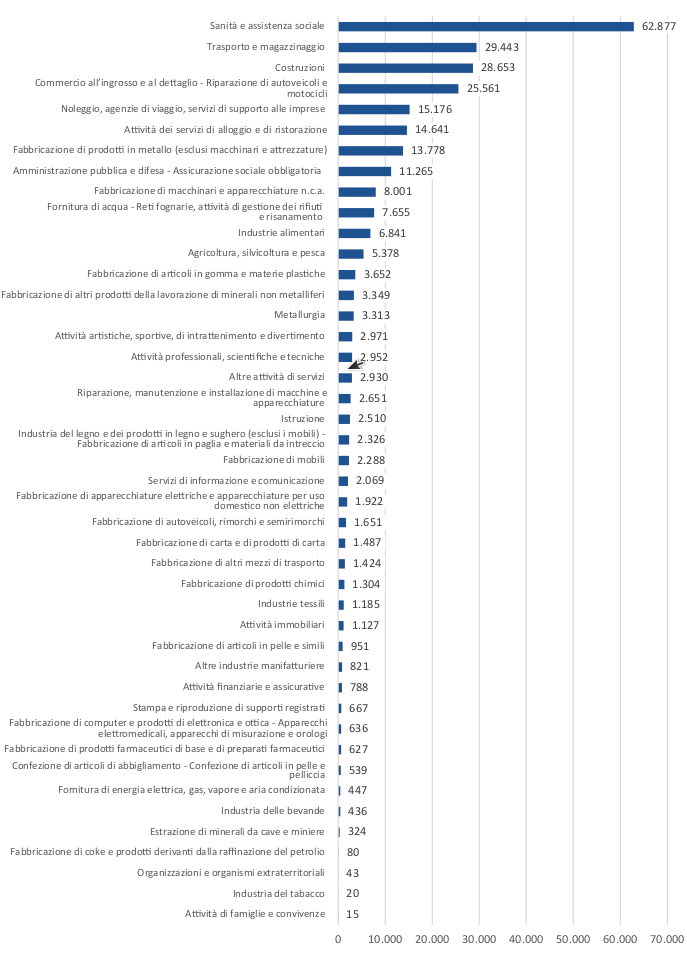
\includegraphics[width=0.8\textwidth]{figures/infortuni_industria_e_servizi.png}
    \caption{infortuni in occasione di lavoro accertati positivi per settore di attività nell'anno 2022}
    \label{fig:infortot}
\end{figure}

Essi comportano gravi conseguenze per i dipendenti, inclusi infortuni permanenti, invalidità e, nei casi più gravi, decessi. Oltre al costo umano, gli incidenti sul lavoro hanno un impatto significativo sull'economia delle aziende, generando costi diretti come spese mediche e indennità di infortunio, e costi indiretti come perdita di produttività, danni reputazionali e aumento dei premi assicurativi. L'EU-Occupational Safety and Health Administration (EU-OSHA) a questo proposito ha stimato in due diversi approcci l'impatto degli incidenti sul lavoro all'interno dell'Unione Europea\cite{osha-eu}. Nell'indagine sono stati presi in esame i dati relativi a 5 Paesi, poiché più completi e accessibili, tra cui figura anche l'Italia e sono stati mostrati i risultati seguendo due diversi approcci: uno bottom-up, perché prende i valori dei costi per ciascun infortunio e li valuta globalmente; l'altro top-down, in quanto stima stima l'impatto dell'infortunio sulla vita del lavoratore e da valori macroeconomici come il PIL pro-capite valuta il costo effettivo dell'infortunio sul singolo. In termini pratici, nel primo caso si tiene conto dei costi diretti, indiretti e immateriali (effetti sulla vita e sulla salute) mentre nel secondo del valore monetario espresso in DALY, cioè il costo in termini di anni di vita persi a causa di un infortunio o di una malattia.

\vspace{0,5cm}
\begin{figure}[htbp]
    \centering
    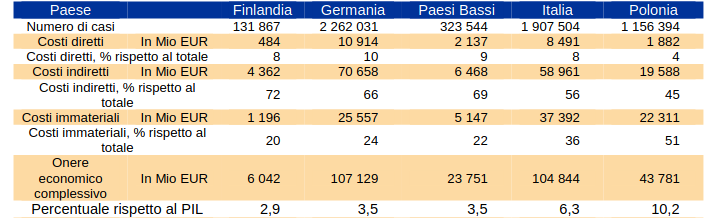
\includegraphics[width=\textwidth]{figures/onere_infortuni_ba.png}
    \caption{onere economico complessivo stimato (approccio bottom up)}
    \label{fig:osha_table1}
\end{figure}
\vspace{0,5cm} 

\noindent Il risultato di queste analisi ha mostrato che per l'Italia il costo di un infortunio o malattia causata dal posto di lavoro aveva un impatto percentuale sul PIL del 6,3\% nel primo caso, mentre nell'approccio top down, riferendosi alla metodologia VSLY - considerata più coerente con i risultati dell'approccio bottom up - il valore medio era del 7,7\% rispetto alla produzione interna. Da questi valori quindi si può dedurre quanto questo problema sia reale e impatti sulla società e sull'economia dell'Italia, dove il posto di lavoro è in gran parte costituito dall'industria. 
 
\begin{figure}[H]
    \centering
    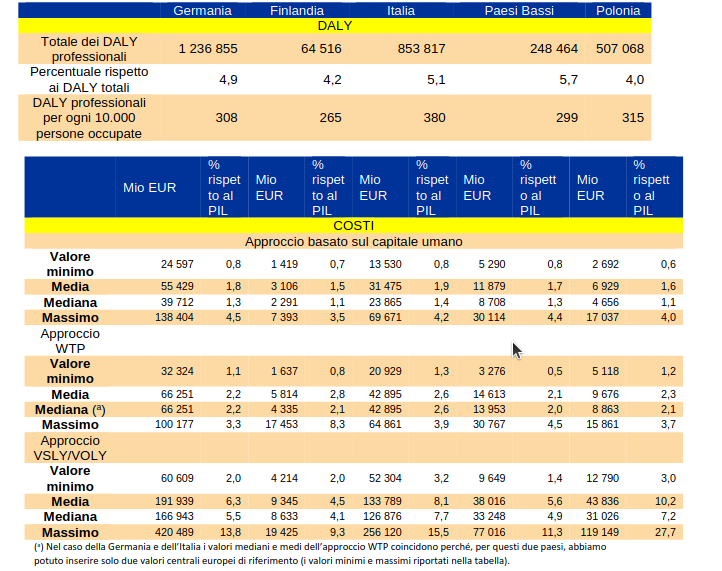
\includegraphics[width=0.8\textwidth]{figures/onere_infortuni_td.png}
    \caption{stima dei costi complessivi approccio top down}
    \label{fig:osha_table2}
\end{figure} 

**********da revisionare***********************************************************
\noindent L'utilizzo corretto dei Dispositivi di Protezione Individuale (DPI) è fondamentale per prevenire tali incidenti. I DPI sono strumenti progettati per proteggere i lavoratori da rischi specifici presenti nell'ambiente di lavoro. Tra i DPI più comuni nell' industria manifatturiera troviamo:

\begin{itemize}
    \item \textbf{Caschi Protettivi}: Proteggono la testa da urti, cadute di oggetti e altre lesioni fisiche. Sono essenziali in ambienti dove operano macchinari pesanti o dove vi è rischio di caduta di materiali.
    \item \textbf{Guanti Protettivi}: Offrono protezione alle mani contro tagli, abrasioni, sostanze chimiche e alte temperature. La scelta del tipo di guanto dipende dal rischio specifico presente nell'ambiente di lavoro.
    \item \textbf{Occhiali Protettivi}: Proteggono gli occhi da particelle volanti, spruzzi di sostanze chimiche e radiazioni nocive. Sono indispensabili in operazioni di taglio, saldatura e manipolazione di materiali pericolosi.
    \item \textbf{Indumenti di Protezione}: Comprendono tute, grembiuli e abbigliamento resistente al fuoco, progettati per proteggere il corpo dai rischi specifici dell'ambiente industriale.
    \item \textbf{Protezioni Uditive}: Come tappi per le orecchie e cuffie antirumore, utilizzate in ambienti con livelli elevati di rumore per prevenire danni all'udito \cite{dpisicurezza}.
    \item \textbf{Mascherine Respiratorie}: Proteggono dalle polveri sottili, vapori e gas nocivi, fondamentali in operazioni di saldatura, verniciatura e manipolazione di sostanze chimiche.
\end{itemize}

L'efficacia dei DPI dipende dall'uso corretto e dalla loro manutenzione regolare. È fondamentale che i lavoratori ricevano una formazione adeguata sull'uso e l'importanza dei DPI, e che le aziende garantiscano la disponibilità di DPI adeguati e in buono stato. Inoltre, i DPI devono essere sostituiti periodicamente e ispezionati per garantirne l’integrità e la funzionalità \cite{dpisicurezza}.

Le normative vigenti in Italia, principalmente il Decreto Legislativo 81/2008, noto come Testo Unico sulla Sicurezza sul Lavoro, regolamentano l'uso dei DPI \cite{decreto81}. Questo decreto stabilisce le disposizioni generali per la tutela della salute e della sicurezza dei lavoratori, specificando le responsabilità dei datori di lavoro nell'analisi dei rischi e nella fornitura di DPI appropriati. Secondo l'articolo 77, i datori di lavoro devono fornire ai lavoratori i DPI necessari per proteggersi dai rischi identificati, garantendo che siano adeguati al tipo di attività svolta e conformi alle normative vigenti.

Il Decreto 81/2008 stabilisce inoltre che i DPI devono essere utilizzati come ultima linea di difesa, dopo aver adottato misure di prevenzione e protezione collettive. Questo principio di gerarchia delle misure di prevenzione sottolinea l'importanza di eliminare o ridurre i rischi a monte prima di affidarsi ai DPI. Inoltre, il decreto prevede che i DPI siano forniti gratuitamente ai lavoratori, che devono essere informati e formati sull'uso corretto degli stessi, e che venga effettuata una valutazione periodica della loro efficacia e conformità \cite{decreto81}.

Le aziende hanno l'obbligo legale di garantire la sicurezza e la salute dei propri dipendenti, conformemente alle leggi nazionali e alle direttive europee. Questo obbligo non è solo un dovere giuridico, ma anche un imperativo morale che riflette l'etica aziendale e il rispetto per la dignità umana. La mancata osservanza delle normative sulla sicurezza può comportare gravi conseguenze legali, incluse sanzioni economiche e responsabilità penali in caso di incidenti gravi \cite{decreto81}.

Sul piano morale, le aziende hanno la responsabilità di proteggere i propri lavoratori non solo per adempiere agli obblighi legali, ma anche per promuovere un ambiente di lavoro sano e sicuro che favorisca il benessere e la produttività. Un impegno serio nella sicurezza sul lavoro contribuisce a costruire una cultura aziendale positiva, migliorando la motivazione e la fidelizzazione dei dipendenti, e rafforzando la reputazione dell'azienda sul mercato \cite{valoresicurezza}.

In conclusione, la sicurezza industriale e l'uso corretto dei DPI sono elementi fondamentali per prevenire gli incidenti sul lavoro e proteggere la salute dei lavoratori nell' industria manifatturiera. Le aziende devono adottare un approccio proattivo nella gestione della sicurezza, combinando misure di prevenzione collettive con l'uso appropriato dei DPI, e rispettando rigorosamente le normative vigenti. Solo attraverso un impegno costante e un'attenzione continua alla sicurezza si può garantire un ambiente di lavoro sicuro ed efficiente, a beneficio sia dei lavoratori che delle aziende stesse.
*****************************************

\section{Computer Vision e Sicurezza sul Lavoro}

Si introdurrà il concetto di computer vision, spiegando come questa tecnologia permetta alle macchine di interpretare e comprendere le immagini. 



Verranno discusse le applicazioni della computer vision nella sicurezza sul lavoro, come il monitoraggio automatico dell'uso dei DPI e la prevenzione degli incidenti attraverso l'analisi in tempo reale.

\section{Cloud Computing nell'Industria}

In questa sezione verrà presentato il cloud computing come modello di erogazione di servizi IT. Si evidenzieranno i vantaggi in termini di scalabilità, flessibilità e riduzione dei costi infrastrutturali. Si collegherà il concetto all'Industria 4.0, spiegando come il cloud sia un elemento chiave per lo sviluppo di fabbriche intelligenti e connesse.

\section{Amazon Rekognition}

Si descriverà in dettaglio il servizio Amazon Rekognition, sottolineando le sue capacità di analisi delle immagini e dei video attraverso algoritmi di deep learning. Si spiegherà come il servizio possa essere utilizzato per il riconoscimento di oggetti, volti e scene, e perché è particolarmente adatto per il rilevamento dei DPI.

\section{Normative e Standard di Sicurezza}

Questo paragrafo esaminerà le principali normative internazionali e nazionali sulla sicurezza sul lavoro, come le direttive europee e le leggi locali. Si discuterà l'importanza della conformità a questi standard e come le tecnologie avanzate possano aiutare le aziende a rispettare le normative e a migliorare la sicurezza complessiva.
